\section{Esercizio19}
\lstinputlisting[language=Matlab]{CodiceMatlab/Esercizio15-19/scriptEs19.m}
Eseguendo lo script si ottiene il seguente grafico:
\begin{figure}[h]
    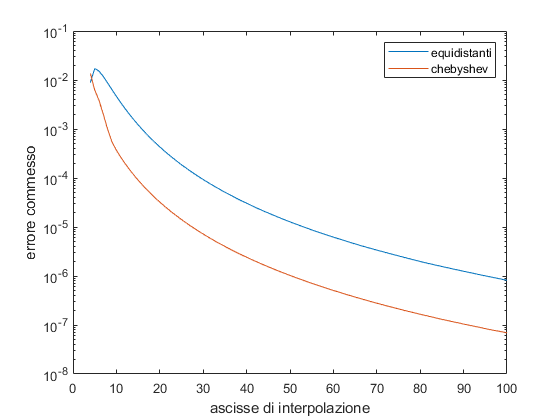
\includegraphics[scale=0.8]{CodiceMatlab/Esercizio15-19/graficoEs19.png}
    \caption{Grafico esercizio 19}
    \label{fig:es19}    
\end{figure}

Confrontando i due grafici possiamo notare che la funzione spline di Matlab commette un errore minore rispetto a splinenat. 
\begin{itemize}
\item Asisse di Chebyshev
 I grafici presentano un'andamento molto simile formando una curva che parte da $10^{-2}$ a $10^{-7}$, essendo l'errore commesso dalla funzione spline leggermente minore.
\item Ascisse equidistanti
Dai grafici si può osservare che utilizzando ascisse equidistanti la funzione splinenat commente un'errore notevolmente maggiore rispetto alla funzione spline di Matlab: nel caso della splinenat l'errore varia da $10^{-1}$ a $10^{-4}$,mentre nel caso della spline di matlab l'errore varia da circa $10^{-2}$ a $10^{-6}$.
\end{itemize}